\DeclareUnicodeCharacter{041B}{\CYRL}



\documentclass[11pt]{article}

    
    
    \usepackage[breakable]{tcolorbox}
    \usepackage{parskip} % Stop auto-indenting (to mimic markdown behaviour)
    \usepackage[english,russian]{babel}
    \usepackage{graphicx}
    \usepackage{subcaption}
    

    % Basic figure setup, for now with no caption control since it's done
    % automatically by Pandoc (which extracts ![](path) syntax from Markdown).
    \usepackage{graphicx}
    % Maintain compatibility with old templates. Remove in nbconvert 6.0
    \let\Oldincludegraphics\includegraphics
    % Ensure that by default, figures have no caption (until we provide a
    % proper Figure object with a Caption API and a way to capture that
    % in the conversion process - todo).
    \usepackage{caption}
    \DeclareCaptionFormat{nocaption}{}
    \captionsetup{format=nocaption,aboveskip=0pt,belowskip=0pt}

    \usepackage{float}
    \floatplacement{figure}{H} % forces figures to be placed at the correct location
    \usepackage{xcolor} % Allow colors to be defined
    \usepackage{enumerate} % Needed for markdown enumerations to work
    \usepackage{geometry} % Used to adjust the document margins
    \usepackage{amsmath} % Equations
    \usepackage{amssymb} % Equations
    \usepackage{textcomp} % defines textquotesingle
    % Hack from http://tex.stackexchange.com/a/47451/13684:
    \AtBeginDocument{%
        \def\PYZsq{\textquotesingle}% Upright quotes in Pygmentized code
    }
    \usepackage{upquote} % Upright quotes for verbatim code
    \usepackage{eurosym} % defines \euro

    \usepackage{iftex}
    \ifPDFTeX
        \usepackage[T1]{fontenc}
        \IfFileExists{alphabeta.sty}{
              \usepackage{alphabeta}
          }{
              \usepackage[mathletters]{ucs}
              \usepackage[utf8x]{inputenc}
          }
    \else
        \usepackage{fontspec}
        \usepackage{unicode-math}
    \fi

    \usepackage{fancyvrb} % verbatim replacement that allows latex
    \usepackage{grffile} % extends the file name processing of package graphics
                         % to support a larger range
    \makeatletter % fix for old versions of grffile with XeLaTeX
    \@ifpackagelater{grffile}{2019/11/01}
    {
      % Do nothing on new versions
    }
    {
      \def\Gread@@xetex#1{%
        \IfFileExists{"\Gin@base".bb}%
        {\Gread@eps{\Gin@base.bb}}%
        {\Gread@@xetex@aux#1}%
      }
    }
    \makeatother
    \usepackage[Export]{adjustbox} % Used to constrain images to a maximum size
    \adjustboxset{max size={0.9\linewidth}{0.9\paperheight}}

    % The hyperref package gives us a pdf with properly built
    % internal navigation ('pdf bookmarks' for the table of contents,
    % internal cross-reference links, web links for URLs, etc.)
    \usepackage{hyperref}
    % The default LaTeX title has an obnoxious amount of whitespace. By default,
    % titling removes some of it. It also provides customization options.
    \usepackage{titling}
    \usepackage{longtable} % longtable support required by pandoc >1.10
    \usepackage{booktabs}  % table support for pandoc > 1.12.2
    \usepackage{array}     % table support for pandoc >= 2.11.3
    \usepackage{calc}      % table minipage width calculation for pandoc >= 2.11.1
    \usepackage[inline]{enumitem} % IRkernel/repr support (it uses the enumerate* environment)
    \usepackage[normalem]{ulem} % ulem is needed to support strikethroughs (\sout)
                                % normalem makes italics be italics, not underlines
    \usepackage{mathrsfs}
    

    
    % Colors for the hyperref package
    \definecolor{urlcolor}{rgb}{0,.145,.698}
    \definecolor{linkcolor}{rgb}{.71,0.21,0.01}
    \definecolor{citecolor}{rgb}{.12,.54,.11}

    % ANSI colors
    \definecolor{ansi-black}{HTML}{3E424D}
    \definecolor{ansi-black-intense}{HTML}{282C36}
    \definecolor{ansi-red}{HTML}{E75C58}
    \definecolor{ansi-red-intense}{HTML}{B22B31}
    \definecolor{ansi-green}{HTML}{00A250}
    \definecolor{ansi-green-intense}{HTML}{007427}
    \definecolor{ansi-yellow}{HTML}{DDB62B}
    \definecolor{ansi-yellow-intense}{HTML}{B27D12}
    \definecolor{ansi-blue}{HTML}{208FFB}
    \definecolor{ansi-blue-intense}{HTML}{0065CA}
    \definecolor{ansi-magenta}{HTML}{D160C4}
    \definecolor{ansi-magenta-intense}{HTML}{A03196}
    \definecolor{ansi-cyan}{HTML}{60C6C8}
    \definecolor{ansi-cyan-intense}{HTML}{258F8F}
    \definecolor{ansi-white}{HTML}{C5C1B4}
    \definecolor{ansi-white-intense}{HTML}{A1A6B2}
    \definecolor{ansi-default-inverse-fg}{HTML}{FFFFFF}
    \definecolor{ansi-default-inverse-bg}{HTML}{000000}

    % common color for the border for error outputs.
    \definecolor{outerrorbackground}{HTML}{FFDFDF}

    % commands and environments needed by pandoc snippets
    % extracted from the output of `pandoc -s`
    \providecommand{\tightlist}{%
      \setlength{\itemsep}{0pt}\setlength{\parskip}{0pt}}
    \DefineVerbatimEnvironment{Highlighting}{Verbatim}{commandchars=\\\{\}}
    % Add ',fontsize=\small' for more characters per line
    \newenvironment{Shaded}{}{}
    \newcommand{\KeywordTok}[1]{\textcolor[rgb]{0.00,0.44,0.13}{\textbf{{#1}}}}
    \newcommand{\DataTypeTok}[1]{\textcolor[rgb]{0.56,0.13,0.00}{{#1}}}
    \newcommand{\DecValTok}[1]{\textcolor[rgb]{0.25,0.63,0.44}{{#1}}}
    \newcommand{\BaseNTok}[1]{\textcolor[rgb]{0.25,0.63,0.44}{{#1}}}
    \newcommand{\FloatTok}[1]{\textcolor[rgb]{0.25,0.63,0.44}{{#1}}}
    \newcommand{\CharTok}[1]{\textcolor[rgb]{0.25,0.44,0.63}{{#1}}}
    \newcommand{\StringTok}[1]{\textcolor[rgb]{0.25,0.44,0.63}{{#1}}}
    \newcommand{\CommentTok}[1]{\textcolor[rgb]{0.38,0.63,0.69}{\textit{{#1}}}}
    \newcommand{\OtherTok}[1]{\textcolor[rgb]{0.00,0.44,0.13}{{#1}}}
    \newcommand{\AlertTok}[1]{\textcolor[rgb]{1.00,0.00,0.00}{\textbf{{#1}}}}
    \newcommand{\FunctionTok}[1]{\textcolor[rgb]{0.02,0.16,0.49}{{#1}}}
    \newcommand{\RegionMarkerTok}[1]{{#1}}
    \newcommand{\ErrorTok}[1]{\textcolor[rgb]{1.00,0.00,0.00}{\textbf{{#1}}}}
    \newcommand{\NormalTok}[1]{{#1}}

    % Additional commands for more recent versions of Pandoc
    \newcommand{\ConstantTok}[1]{\textcolor[rgb]{0.53,0.00,0.00}{{#1}}}
    \newcommand{\SpecialCharTok}[1]{\textcolor[rgb]{0.25,0.44,0.63}{{#1}}}
    \newcommand{\VerbatimStringTok}[1]{\textcolor[rgb]{0.25,0.44,0.63}{{#1}}}
    \newcommand{\SpecialStringTok}[1]{\textcolor[rgb]{0.73,0.40,0.53}{{#1}}}
    \newcommand{\ImportTok}[1]{{#1}}
    \newcommand{\DocumentationTok}[1]{\textcolor[rgb]{0.73,0.13,0.13}{\textit{{#1}}}}
    \newcommand{\AnnotationTok}[1]{\textcolor[rgb]{0.38,0.63,0.69}{\textbf{\textit{{#1}}}}}
    \newcommand{\CommentVarTok}[1]{\textcolor[rgb]{0.38,0.63,0.69}{\textbf{\textit{{#1}}}}}
    \newcommand{\VariableTok}[1]{\textcolor[rgb]{0.10,0.09,0.49}{{#1}}}
    \newcommand{\ControlFlowTok}[1]{\textcolor[rgb]{0.00,0.44,0.13}{\textbf{{#1}}}}
    \newcommand{\OperatorTok}[1]{\textcolor[rgb]{0.40,0.40,0.40}{{#1}}}
    \newcommand{\BuiltInTok}[1]{{#1}}
    \newcommand{\ExtensionTok}[1]{{#1}}
    \newcommand{\PreprocessorTok}[1]{\textcolor[rgb]{0.74,0.48,0.00}{{#1}}}
    \newcommand{\AttributeTok}[1]{\textcolor[rgb]{0.49,0.56,0.16}{{#1}}}
    \newcommand{\InformationTok}[1]{\textcolor[rgb]{0.38,0.63,0.69}{\textbf{\textit{{#1}}}}}
    \newcommand{\WarningTok}[1]{\textcolor[rgb]{0.38,0.63,0.69}{\textbf{\textit{{#1}}}}}


    % Define a nice break command that doesn't care if a line doesn't already
    % exist.
    \def\br{\hspace*{\fill} \\* }
    % Math Jax compatibility definitions
    \def\gt{>}
    \def\lt{<}
    \let\Oldtex\TeX
    \let\Oldlatex\LaTeX
    \renewcommand{\TeX}{\textrm{\Oldtex}}
    \renewcommand{\LaTeX}{\textrm{\Oldlatex}}
    % Document parameters
    % Document title
    \title{CHM\_Lab1}
    
    
    
    
    
% Pygments definitions
\makeatletter
\def\PY@reset{\let\PY@it=\relax \let\PY@bf=\relax%
    \let\PY@ul=\relax \let\PY@tc=\relax%
    \let\PY@bc=\relax \let\PY@ff=\relax}
\def\PY@tok#1{\csname PY@tok@#1\endcsname}
\def\PY@toks#1+{\ifx\relax#1\empty\else%
    \PY@tok{#1}\expandafter\PY@toks\fi}
\def\PY@do#1{\PY@bc{\PY@tc{\PY@ul{%
    \PY@it{\PY@bf{\PY@ff{#1}}}}}}}
\def\PY#1#2{\PY@reset\PY@toks#1+\relax+\PY@do{#2}}

\@namedef{PY@tok@w}{\def\PY@tc##1{\textcolor[rgb]{0.73,0.73,0.73}{##1}}}
\@namedef{PY@tok@c}{\let\PY@it=\textit\def\PY@tc##1{\textcolor[rgb]{0.24,0.48,0.48}{##1}}}
\@namedef{PY@tok@cp}{\def\PY@tc##1{\textcolor[rgb]{0.61,0.40,0.00}{##1}}}
\@namedef{PY@tok@k}{\let\PY@bf=\textbf\def\PY@tc##1{\textcolor[rgb]{0.00,0.50,0.00}{##1}}}
\@namedef{PY@tok@kp}{\def\PY@tc##1{\textcolor[rgb]{0.00,0.50,0.00}{##1}}}
\@namedef{PY@tok@kt}{\def\PY@tc##1{\textcolor[rgb]{0.69,0.00,0.25}{##1}}}
\@namedef{PY@tok@o}{\def\PY@tc##1{\textcolor[rgb]{0.40,0.40,0.40}{##1}}}
\@namedef{PY@tok@ow}{\let\PY@bf=\textbf\def\PY@tc##1{\textcolor[rgb]{0.67,0.13,1.00}{##1}}}
\@namedef{PY@tok@nb}{\def\PY@tc##1{\textcolor[rgb]{0.00,0.50,0.00}{##1}}}
\@namedef{PY@tok@nf}{\def\PY@tc##1{\textcolor[rgb]{0.00,0.00,1.00}{##1}}}
\@namedef{PY@tok@nc}{\let\PY@bf=\textbf\def\PY@tc##1{\textcolor[rgb]{0.00,0.00,1.00}{##1}}}
\@namedef{PY@tok@nn}{\let\PY@bf=\textbf\def\PY@tc##1{\textcolor[rgb]{0.00,0.00,1.00}{##1}}}
\@namedef{PY@tok@ne}{\let\PY@bf=\textbf\def\PY@tc##1{\textcolor[rgb]{0.80,0.25,0.22}{##1}}}
\@namedef{PY@tok@nv}{\def\PY@tc##1{\textcolor[rgb]{0.10,0.09,0.49}{##1}}}
\@namedef{PY@tok@no}{\def\PY@tc##1{\textcolor[rgb]{0.53,0.00,0.00}{##1}}}
\@namedef{PY@tok@nl}{\def\PY@tc##1{\textcolor[rgb]{0.46,0.46,0.00}{##1}}}
\@namedef{PY@tok@ni}{\let\PY@bf=\textbf\def\PY@tc##1{\textcolor[rgb]{0.44,0.44,0.44}{##1}}}
\@namedef{PY@tok@na}{\def\PY@tc##1{\textcolor[rgb]{0.41,0.47,0.13}{##1}}}
\@namedef{PY@tok@nt}{\let\PY@bf=\textbf\def\PY@tc##1{\textcolor[rgb]{0.00,0.50,0.00}{##1}}}
\@namedef{PY@tok@nd}{\def\PY@tc##1{\textcolor[rgb]{0.67,0.13,1.00}{##1}}}
\@namedef{PY@tok@s}{\def\PY@tc##1{\textcolor[rgb]{0.73,0.13,0.13}{##1}}}
\@namedef{PY@tok@sd}{\let\PY@it=\textit\def\PY@tc##1{\textcolor[rgb]{0.73,0.13,0.13}{##1}}}
\@namedef{PY@tok@si}{\let\PY@bf=\textbf\def\PY@tc##1{\textcolor[rgb]{0.64,0.35,0.47}{##1}}}
\@namedef{PY@tok@se}{\let\PY@bf=\textbf\def\PY@tc##1{\textcolor[rgb]{0.67,0.36,0.12}{##1}}}
\@namedef{PY@tok@sr}{\def\PY@tc##1{\textcolor[rgb]{0.64,0.35,0.47}{##1}}}
\@namedef{PY@tok@ss}{\def\PY@tc##1{\textcolor[rgb]{0.10,0.09,0.49}{##1}}}
\@namedef{PY@tok@sx}{\def\PY@tc##1{\textcolor[rgb]{0.00,0.50,0.00}{##1}}}
\@namedef{PY@tok@m}{\def\PY@tc##1{\textcolor[rgb]{0.40,0.40,0.40}{##1}}}
\@namedef{PY@tok@gh}{\let\PY@bf=\textbf\def\PY@tc##1{\textcolor[rgb]{0.00,0.00,0.50}{##1}}}
\@namedef{PY@tok@gu}{\let\PY@bf=\textbf\def\PY@tc##1{\textcolor[rgb]{0.50,0.00,0.50}{##1}}}
\@namedef{PY@tok@gd}{\def\PY@tc##1{\textcolor[rgb]{0.63,0.00,0.00}{##1}}}
\@namedef{PY@tok@gi}{\def\PY@tc##1{\textcolor[rgb]{0.00,0.52,0.00}{##1}}}
\@namedef{PY@tok@gr}{\def\PY@tc##1{\textcolor[rgb]{0.89,0.00,0.00}{##1}}}
\@namedef{PY@tok@ge}{\let\PY@it=\textit}
\@namedef{PY@tok@gs}{\let\PY@bf=\textbf}
\@namedef{PY@tok@gp}{\let\PY@bf=\textbf\def\PY@tc##1{\textcolor[rgb]{0.00,0.00,0.50}{##1}}}
\@namedef{PY@tok@go}{\def\PY@tc##1{\textcolor[rgb]{0.44,0.44,0.44}{##1}}}
\@namedef{PY@tok@gt}{\def\PY@tc##1{\textcolor[rgb]{0.00,0.27,0.87}{##1}}}
\@namedef{PY@tok@err}{\def\PY@bc##1{{\setlength{\fboxsep}{\string -\fboxrule}\fcolorbox[rgb]{1.00,0.00,0.00}{1,1,1}{\strut ##1}}}}
\@namedef{PY@tok@kc}{\let\PY@bf=\textbf\def\PY@tc##1{\textcolor[rgb]{0.00,0.50,0.00}{##1}}}
\@namedef{PY@tok@kd}{\let\PY@bf=\textbf\def\PY@tc##1{\textcolor[rgb]{0.00,0.50,0.00}{##1}}}
\@namedef{PY@tok@kn}{\let\PY@bf=\textbf\def\PY@tc##1{\textcolor[rgb]{0.00,0.50,0.00}{##1}}}
\@namedef{PY@tok@kr}{\let\PY@bf=\textbf\def\PY@tc##1{\textcolor[rgb]{0.00,0.50,0.00}{##1}}}
\@namedef{PY@tok@bp}{\def\PY@tc##1{\textcolor[rgb]{0.00,0.50,0.00}{##1}}}
\@namedef{PY@tok@fm}{\def\PY@tc##1{\textcolor[rgb]{0.00,0.00,1.00}{##1}}}
\@namedef{PY@tok@vc}{\def\PY@tc##1{\textcolor[rgb]{0.10,0.09,0.49}{##1}}}
\@namedef{PY@tok@vg}{\def\PY@tc##1{\textcolor[rgb]{0.10,0.09,0.49}{##1}}}
\@namedef{PY@tok@vi}{\def\PY@tc##1{\textcolor[rgb]{0.10,0.09,0.49}{##1}}}
\@namedef{PY@tok@vm}{\def\PY@tc##1{\textcolor[rgb]{0.10,0.09,0.49}{##1}}}
\@namedef{PY@tok@sa}{\def\PY@tc##1{\textcolor[rgb]{0.73,0.13,0.13}{##1}}}
\@namedef{PY@tok@sb}{\def\PY@tc##1{\textcolor[rgb]{0.73,0.13,0.13}{##1}}}
\@namedef{PY@tok@sc}{\def\PY@tc##1{\textcolor[rgb]{0.73,0.13,0.13}{##1}}}
\@namedef{PY@tok@dl}{\def\PY@tc##1{\textcolor[rgb]{0.73,0.13,0.13}{##1}}}
\@namedef{PY@tok@s2}{\def\PY@tc##1{\textcolor[rgb]{0.73,0.13,0.13}{##1}}}
\@namedef{PY@tok@sh}{\def\PY@tc##1{\textcolor[rgb]{0.73,0.13,0.13}{##1}}}
\@namedef{PY@tok@s1}{\def\PY@tc##1{\textcolor[rgb]{0.73,0.13,0.13}{##1}}}
\@namedef{PY@tok@mb}{\def\PY@tc##1{\textcolor[rgb]{0.40,0.40,0.40}{##1}}}
\@namedef{PY@tok@mf}{\def\PY@tc##1{\textcolor[rgb]{0.40,0.40,0.40}{##1}}}
\@namedef{PY@tok@mh}{\def\PY@tc##1{\textcolor[rgb]{0.40,0.40,0.40}{##1}}}
\@namedef{PY@tok@mi}{\def\PY@tc##1{\textcolor[rgb]{0.40,0.40,0.40}{##1}}}
\@namedef{PY@tok@il}{\def\PY@tc##1{\textcolor[rgb]{0.40,0.40,0.40}{##1}}}
\@namedef{PY@tok@mo}{\def\PY@tc##1{\textcolor[rgb]{0.40,0.40,0.40}{##1}}}
\@namedef{PY@tok@ch}{\let\PY@it=\textit\def\PY@tc##1{\textcolor[rgb]{0.24,0.48,0.48}{##1}}}
\@namedef{PY@tok@cm}{\let\PY@it=\textit\def\PY@tc##1{\textcolor[rgb]{0.24,0.48,0.48}{##1}}}
\@namedef{PY@tok@cpf}{\let\PY@it=\textit\def\PY@tc##1{\textcolor[rgb]{0.24,0.48,0.48}{##1}}}
\@namedef{PY@tok@c1}{\let\PY@it=\textit\def\PY@tc##1{\textcolor[rgb]{0.24,0.48,0.48}{##1}}}
\@namedef{PY@tok@cs}{\let\PY@it=\textit\def\PY@tc##1{\textcolor[rgb]{0.24,0.48,0.48}{##1}}}

\def\PYZbs{\char`\\}
\def\PYZus{\char`\_}
\def\PYZob{\char`\{}
\def\PYZcb{\char`\}}
\def\PYZca{\char`\^}
\def\PYZam{\char`\&}
\def\PYZlt{\char`\<}
\def\PYZgt{\char`\>}
\def\PYZsh{\char`\#}
\def\PYZpc{\char`\%}
\def\PYZdl{\char`\$}
\def\PYZhy{\char`\-}
\def\PYZsq{\char`\'}
\def\PYZdq{\char`\"}
\def\PYZti{\char`\~}
% for compatibility with earlier versions
\def\PYZat{@}
\def\PYZlb{[}
\def\PYZrb{]}
\makeatother


    % For linebreaks inside Verbatim environment from package fancyvrb.
    \makeatletter
        \newbox\Wrappedcontinuationbox
        \newbox\Wrappedvisiblespacebox
        \newcommand*\Wrappedvisiblespace {\textcolor{red}{\textvisiblespace}}
        \newcommand*\Wrappedcontinuationsymbol {\textcolor{red}{\llap{\tiny$\m@th\hookrightarrow$}}}
        \newcommand*\Wrappedcontinuationindent {3ex }
        \newcommand*\Wrappedafterbreak {\kern\Wrappedcontinuationindent\copy\Wrappedcontinuationbox}
        % Take advantage of the already applied Pygments mark-up to insert
        % potential linebreaks for TeX processing.
        %        {, <, #, %, $, ' and ": go to next line.
        %        _, }, ^, &, >, - and ~: stay at end of broken line.
        % Use of \textquotesingle for straight quote.
        \newcommand*\Wrappedbreaksatspecials {%
            \def\PYGZus{\discretionary{\char`\_}{\Wrappedafterbreak}{\char`\_}}%
            \def\PYGZob{\discretionary{}{\Wrappedafterbreak\char`\{}{\char`\{}}%
            \def\PYGZcb{\discretionary{\char`\}}{\Wrappedafterbreak}{\char`\}}}%
            \def\PYGZca{\discretionary{\char`\^}{\Wrappedafterbreak}{\char`\^}}%
            \def\PYGZam{\discretionary{\char`\&}{\Wrappedafterbreak}{\char`\&}}%
            \def\PYGZlt{\discretionary{}{\Wrappedafterbreak\char`\<}{\char`\<}}%
            \def\PYGZgt{\discretionary{\char`\>}{\Wrappedafterbreak}{\char`\>}}%
            \def\PYGZsh{\discretionary{}{\Wrappedafterbreak\char`\#}{\char`\#}}%
            \def\PYGZpc{\discretionary{}{\Wrappedafterbreak\char`\%}{\char`\%}}%
            \def\PYGZdl{\discretionary{}{\Wrappedafterbreak\char`\$}{\char`\$}}%
            \def\PYGZhy{\discretionary{\char`\-}{\Wrappedafterbreak}{\char`\-}}%
            \def\PYGZsq{\discretionary{}{\Wrappedafterbreak\textquotesingle}{\textquotesingle}}%
            \def\PYGZdq{\discretionary{}{\Wrappedafterbreak\char`\"}{\char`\"}}%
            \def\PYGZti{\discretionary{\char`\~}{\Wrappedafterbreak}{\char`\~}}%
        }
        % Some characters . , ; ? ! / are not pygmentized.
        % This macro makes them "active" and they will insert potential linebreaks
        \newcommand*\Wrappedbreaksatpunct {%
            \lccode`\~`\.\lowercase{\def~}{\discretionary{\hbox{\char`\.}}{\Wrappedafterbreak}{\hbox{\char`\.}}}%
            \lccode`\~`\,\lowercase{\def~}{\discretionary{\hbox{\char`\,}}{\Wrappedafterbreak}{\hbox{\char`\,}}}%
            \lccode`\~`\;\lowercase{\def~}{\discretionary{\hbox{\char`\;}}{\Wrappedafterbreak}{\hbox{\char`\;}}}%
            \lccode`\~`\:\lowercase{\def~}{\discretionary{\hbox{\char`\:}}{\Wrappedafterbreak}{\hbox{\char`\:}}}%
            \lccode`\~`\?\lowercase{\def~}{\discretionary{\hbox{\char`\?}}{\Wrappedafterbreak}{\hbox{\char`\?}}}%
            \lccode`\~`\!\lowercase{\def~}{\discretionary{\hbox{\char`\!}}{\Wrappedafterbreak}{\hbox{\char`\!}}}%
            \lccode`\~`\/\lowercase{\def~}{\discretionary{\hbox{\char`\/}}{\Wrappedafterbreak}{\hbox{\char`\/}}}%
            \catcode`\.\active
            \catcode`\,\active
            \catcode`\;\active
            \catcode`\:\active
            \catcode`\?\active
            \catcode`\!\active
            \catcode`\/\active
            \lccode`\~`\~
        }
    \makeatother

    \let\OriginalVerbatim=\Verbatim
    \makeatletter
    \renewcommand{\Verbatim}[1][1]{%
        %\parskip\z@skip
        \sbox\Wrappedcontinuationbox {\Wrappedcontinuationsymbol}%
        \sbox\Wrappedvisiblespacebox {\FV@SetupFont\Wrappedvisiblespace}%
        \def\FancyVerbFormatLine ##1{\hsize\linewidth
            \vtop{\raggedright\hyphenpenalty\z@\exhyphenpenalty\z@
                \doublehyphendemerits\z@\finalhyphendemerits\z@
                \strut ##1\strut}%
        }%
        % If the linebreak is at a space, the latter will be displayed as visible
        % space at end of first line, and a continuation symbol starts next line.
        % Stretch/shrink are however usually zero for typewriter font.
        \def\FV@Space {%
            \nobreak\hskip\z@ plus\fontdimen3\font minus\fontdimen4\font
            \discretionary{\copy\Wrappedvisiblespacebox}{\Wrappedafterbreak}
            {\kern\fontdimen2\font}%
        }%

        % Allow breaks at special characters using \PYG... macros.
        \Wrappedbreaksatspecials
        % Breaks at punctuation characters . , ; ? ! and / need catcode=\active
        \OriginalVerbatim[#1,codes*=\Wrappedbreaksatpunct]%
    }
    \makeatother

    % Exact colors from NB
    \definecolor{incolor}{HTML}{303F9F}
    \definecolor{outcolor}{HTML}{D84315}
    \definecolor{cellborder}{HTML}{CFCFCF}
    \definecolor{cellbackground}{HTML}{F7F7F7}

    % prompt
    \makeatletter
    \newcommand{\boxspacing}{\kern\kvtcb@left@rule\kern\kvtcb@boxsep}
    \makeatother
    \newcommand{\prompt}[4]{
        {\ttfamily\llap{{\color{#2}[#3]:\hspace{3pt}#4}}\vspace{-\baselineskip}}
    }
    

    
    % Prevent overflowing lines due to hard-to-break entities
    \sloppy
    % Setup hyperref package
    \hypersetup{
      breaklinks=true,  % so long urls are correctly broken across lines
      colorlinks=true,
      urlcolor=urlcolor,
      linkcolor=linkcolor,
      citecolor=citecolor,
      }
    % Slightly bigger margins than the latex defaults
    
    \geometry{verbose,tmargin=1in,bmargin=1in,lmargin=1in,rmargin=1in}
    
\newtheorem{theorem}{Теорема}

\begin{document}
    
    \begin{titlepage}
    \newpage
    
    \begin{center}
    МИНИСТЕРСТВО ОБРАЗОВАНИЯ РЕСПУБЛИКИ БЕЛАРУСЬ БЕЛОРУССКИЙ ГОСУДАРСТВЕННЫЙ УНИВЕРСИТЕТ \\
    Факультет прикладной математики и инворматики \\ Кафедра вычислительной математики
 
    \end{center}
    
    \vspace{8em}
    
    \vspace{2em}
    
    \begin{center}
    \textsc{\textbf{Отчет по лабораторной работе 1 \\ "Аппроксимация дифференциальных задач разностными операторами" \linebreak Вариант 5}}
    \end{center}
    
    \vspace{6em}
    
    \begin{flushright}
        Выполнил:\\
        Карпович Артём Дмитриевич\\
        студент 4 курса 7 группы
    \end{flushright}
    
    \begin{flushright}
        Преподаватель:\\
        Репников Василий Иванович
    \end{flushright}
    
    \vspace{\fill}
    
    \vspace{\fill}
    
    \begin{center}
    Минск, 2024
    \end{center}
    
    \end{titlepage}
    

    \section*{Постановка
задач}\label{ux43fux43eux441ux442ux430ux43dux43eux432ux43aux430-ux437ux430ux434ux430ux447}
\begin{enumerate}
    \item Построить разностную аппроксимацию оператора Lu методом неопределенных коэффициентов, где $$Lu=u'(x_1);$$
    \begin{figure}
        \centering
        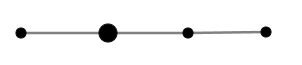
\includegraphics[width=0.35\linewidth]{image1.png}
    \end{figure}
    \item Построить разностную аппроксимацию оператора Lu методом неопределенных коэффициентов, где $$Lu=\frac{\partial^2 u(x_1,x_2)}{\partial x_1^2};$$
    \begin{figure}
        \centering
        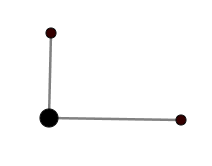
\includegraphics[width=0.25\linewidth]{image2.png}
    \end{figure}
    \item Аппроксимировать дифференциальную задачу разностной схемой на заданном шаблоне. Опеределить погрешность аппроксимации;
    \item Повысить порядок аппроксимации разностной схемы на минимальном шаблоне, используя вид дифференциальной задачи.
\end{enumerate}
$$3,4.\begin{cases}
    \frac{\partial^2 u}{\partial t^2}=\frac{\partial^2 u}{\partial x^2}+q(x,t)u+f(x,t), 0<x<1,t>0,\\
    u(x,0)=u_0(x),\frac{\partial u(x,0)}{\partial t}=u_1(x,t), 0 \leq x \leq 1,\\
    \frac{\partial u(0,t)}{\partial x}=\sigma_0 u(0,t)-\mu_0(t),u(1,t)=\mu_1(t),t\geq0.
\end{cases}$$
\begin{figure}
    \centering
    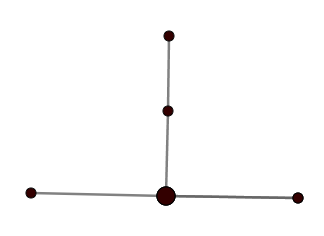
\includegraphics[width=0.35\linewidth]{image3.png}
\end{figure}
\newpage

\subsection*{Задача 1}
\textbf{Постановка задачи.} Построить разностную аппроксимацию оператора Lu методом неопределенных коэффициентов, где $$Lu=u'(x_1);$$
    \begin{figure}
        \centering
        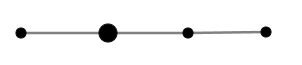
\includegraphics[width=0.35\linewidth]{image1.png}
    \end{figure}
\textbf{Решение задачи.}Рассмотрим равномерную сетку узлов с шагом $h$. И введем следующие обозначения: $$x=x_1, \Rightarrow x_0=x-h, x_2=x+h, x_3=x+2h$$
Тогда наш шаблон примет вид $$\text{Ш}(x)=\{x-h,x,x+h,x+2h\}.$$
Разностную аппроксимацию будем искать в виде линейной комбинации значений функции
$u$ в точках шаблона, то есть: $$L_hu(x)=a_0u(x-h)+a_1u(x)+a_2u(x+h)+a_3u(x+2h).$$
Выпишем погрешность нашей аппроксимации: $$\psi(x)=L_hu(x)-Lu(x)=a_0u(x-h)+a_1u(x)+a_2u(x+h)+a_3u(x+2h)-u'(x).$$
Разложим правую часть этого выражения в ряд Тейлора в окрестности точки $x$:
$$\psi(x)=a_0(u-hu'+\frac{h^2}{2}u''-\frac{h^3}{6}u''')+a_1u+a_2(u+hu'+\frac{h^2}{2}u''+\frac{h^3}{6}u''')+a_3(u+2hu'+2h^2u''+\frac{4h^3}{3}u''')+O(h^4)-u'=$$
$$=(a_0+a_1+a_2+a_3)u-h(a_0-a_2-2a-3+\frac{1}{h})u'+\frac{h^2}{2}(a_0+a_2+4a_3)u''+\frac{h^3}{6}(-a_0+a_2+8a_3)u'''+O(h^4).$$
Для того, чтобы погрешность аппроксимации была минимальной, необходимо, чтобы коэффициенты при производных должны быть равны нулю, таким образом, мы можем сформировать систему для поиска коэффициентов $a_k$:
$$\begin{cases}
    a_0+a_1+a_2+a_3=0,\\
    a_0-a_2-2a-3+\frac{1}{h}=0,\\
    a_0+a_2+4a_3=0,\\
    -a_0+a_2+8a_3=0.
\end{cases}$$
Выразим из третьего уравнения $a_0$ и выполним подстановку во все уравнения:
$$\begin{cases}
    a_0=-4a_3-a_2,\\
    a_1-3a_3=0,\\
    a_2+3a_3=\frac{1}{2h},\\
    a_2+6a_3=0,
\end{cases}\Rightarrow [\text{Выражаем из последнего $a_2$}]\Rightarrow
\begin{cases}
    a_2=-6a_3,\\
    a_0=2a_3,\\
    a_1=3a_3,\\
    3a_3=-\frac{1}{2h},
\end{cases} \Rightarrow
\begin{cases}
    a_0=-\frac{1}{3h},\\
    a_1=-\frac{1}{2h},\\
    a_2=\frac{1}{h},\\
    a_3=-\frac{1}{6h}.
\end{cases}$$
Таким образом, мы нашли коэффициенты, с помощью которых можем построить разностную аппроксимацию оператора $Lu=u'(x)$:
$$L_hu=-\frac{1}{h}(\dfrac13 u(x-h)+\dfrac12 u(x)-u(x+h)+\dfrac16 u(x+2h)).$$
\newpage

\subsection*{Задача 2}
\textbf{Постановка задачи}.Построить разностную аппроксимацию оператора Lu методом неопределенных коэффициентов, где $$Lu=\frac{\partial^2 u(x_1,x_2)}{\partial x_1^2};$$
    \begin{figure}
        \centering
        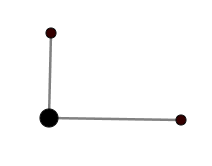
\includegraphics[width=0.25\linewidth]{image2.png}
    \end{figure}
    
\textbf{Решение задачи.} Разностную аппроксимацию будем искать в виде линейной комбинации значений функции
$u$ в точках шаблона, то есть: $$L_hu(x)=a_0u(x_1,x_2)+a_1u(x_1,x_2+h_2)+a_2u(x_1+h_1,x_2).$$
Выпишем погрешность нашей аппроксимации: $$\psi(x)=a_0u(x_1,x_2)+a_1u(x_1,x_2+h_2)+a_2u(x_1+h_1,x_2)-\frac{\partial^2 u(x_1,x_2)}{\partial x_1^2}.$$
Разложим правую часть этого выражения в ряд Тейлора, используя формулу разложения функции двух переменных:
$$\psi(x)=a_0u+a_1(u+h_2\frac{\partial u}{\partial x_2}+\frac{h_2^2}{2}\frac{\partial^2 u}{\partial x_2^2})+a_2(u+h_1\frac{\partial u}{\partial x_1}+\frac{h_1^2}{2}\frac{\partial^2 u}{\partial x_1^2})+O(h^3)-\frac{\partial^2 u(x_1,x_2)}{\partial x_1^2}=(a_0+a_1+a_2)u+$$
$$+h_1a_2\frac{\partial u}{\partial x_1}+h_2a_1 \frac{\partial u}{\partial x_2}+\frac{h_2^2}{2}a_1\frac{\partial^2 u}{\partial x_2^2}+\frac{h_1^2}{2}(a_2-\frac{2}{h_1^2})\frac{\partial^2 u}{\partial x_1^2}+O(h^3).$$
Для того, чтобы погрешность аппроксимации была минимальной, необходимо, чтобы коэффициенты при производных должны быть равны нулю, таким образом, мы можем сформировать систему для поиска коэффициентов $a_k$:
$$\begin{cases}
    a_0+a_1+a_2=0,\\
    a_2=0,\\
    a_1=0,\\
    a_2=\frac{2}{h_1^2}.
\end{cases}$$
Как можно заметить, мы получили некое противоречие, что можно объяснить тем, что наш шаблон не удовлетворяет нашей задаче, посколько нам для аппроксимации второй производной необходимо по крайней мере три точки, а на даны лишь две точки, помимо центральной. 

Таким образом, можно сделать вид, что для нашего оператора на данном шаблоне построить разностную аппроксимацию невозможно.
\newpage
\subsection*{Задача 3}
\textbf{Постановка задачи.} Аппроксимировать дифференциальную задачу разностной схемой на заданном шаблоне.
Опеределить погрешность аппроксимации;
$$\begin{cases}
    \frac{\partial^2 u}{\partial t^2}=\frac{\partial^2 u}{\partial x^2}+q(x,t)u+f(x,t), 0<x<1,t>0,\\
    u(x,0)=u_0(x),\frac{\partial u(x,0)}{\partial t}=u_1(x), 0 \leq x \leq 1,\\
    \frac{\partial u(0,t)}{\partial x}=\sigma_0 u(0,t)-\mu_0(t),u(1,t)=\mu_1(t),t\geq0.
\end{cases}$$
\begin{figure}
    \centering
    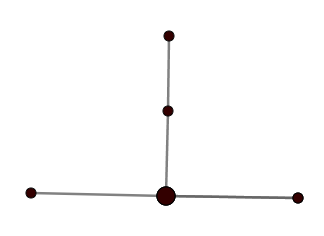
\includegraphics[width=0.35\linewidth]{image3.png}
\end{figure}
\textbf{Решение.} Запишем рассматриваемую задачу в безиндексной форме:
$$\begin{cases}
    y_{tt}=y_{\overline{x} x}+qy+f, x,t\in \omega_{h\tau},\\
    y(x,0)=u_0(x),\\
    y_t(x,0)=u_1(x), \\
    y_x(0,t)=\sigma_0 y(0,t)-\mu_0(t),\\
    y(1,t)=\mu_1(t),
\end{cases}$$
где $\omega_{h\tau} -$ сетка рассматриваемых узлов. 

Построим разностную аппроксимацию для оператора $Lu=\frac{\partial^2 u}{\partial t^2}$ с помощью метода неопределенных коэффициентов аналогично тому, как делали это во втором задании. Для этого воспользуемся представлением в виде линейной комбинации значений функции $u$ в точках шаблона:
$$L_h u(x,t)=a_0u(x,t)+a_1u(x,t+\tau)+a_2u(x,t+2\tau)$$
Выпишем погрешность аппроксимации:
$$\psi(x,t)=L_hu-Lu=a_0u(x,t)+a_1u(x,t+\tau)+a_2u(x,t+2\tau)-\frac{\partial^2 u}{\partial t^2}.$$
Разложим данное выражение в ряд Тейлора, сразу приводя подобные:
$$\psi(x,t)=(a_0+a_1+a_2)u+\tau(a_1+2a_2)\frac{\partial u}{\partial t}+\tau^2(\frac{a_1}{2}+2a_2-\frac{1}{\tau^2})\frac{\partial^2 u}{\partial \tau^2}+O(\tau^3).$$
Аналогично первым двум заданиям, строим систему для зануления коэффициентов:
$$\begin{cases}
    a_0+a_1+a_2=0,\\
    a_1+2a_2=0,\\
    \frac{a_1}{2}+2a_2-\frac{1}{\tau^2}=0,
\end{cases}\Rightarrow
\begin{cases}
    a_0=\frac{1}{\tau^2},\\
    a_1=-\frac{2}{\tau^2},\\
    a_2=\frac{1}{\tau^2}.
\end{cases}$$
Таким образом, вторая разностная производная принимает вид:
$$L_hu(x,t)=\frac{u(x,t)-2u(x,t+\tau)+u(x,t+2\tau)}{\tau^2}.$$
Используя получившееся выражение, запишем нашу задачу в индексной форме:
$$\begin{cases}
    \frac{y_i^{j+2}-2y_i^{j+1}+y_{i}^j}{\tau^2}=\frac{y_{i+1}^j-2y_i^j+y_{i-1}^j}{h^2}+q(x_i,t_j)y_i^j+f(x_i,t_j),i=\overline{1,N-1},\\
    y_i^0=u_0(x_i),\\
    \frac{y_{i+1}^1-y_{i+1}^0}{h}=u_1(x),\\
    \frac{y_{1}^{j+1}-y_{0}^{j+1}}{h}=\sigma_0 y_0^{j}-\mu_0(t_j),\\
    y_{1}^{j+1}=\mu_1(t_j)
\end{cases}$$
Таким образом, мы получили разностную схему данной задачи. Перейдем к определению погрешности аппроксимации.
$$\psi(x,t)=\frac{u(x,t)-2u(x,t+\tau)+u(x,t+2\tau)}{\tau^2}-u_{\overline{x}x}-q(x,t)u-f(x,t).$$
Разложим в ряд Тейлора почленно:
$$\frac{u(x,t)-2u(x,t+\tau)+u(x,t+2\tau)}{\tau^2}=\frac{1}{\tau^2}(u-2(u+\tau\frac{\partial u}{\partial t}+\frac{\tau^2}{2}\frac{\partial^2 u}{\partial t^2}+\frac{\tau^3}{6}\frac{\partial^3 u}{\partial t^3})+u+2\tau \frac{\partial u}{\partial t}+2\tau^2 \frac{\partial^2 u}{\partial t^2}+\frac{4\tau^3}{3}\frac{\partial^3 u}{\partial t^3}+$$
$$+O(\tau^4))=\frac{1}{\tau^2}(\tau^3\frac{\partial^3 u}{\partial t^3}+O(\tau^4))=O(\tau).$$
$$u_{\overline{x}x}=[\text{выводили на паре}]=\frac{\partial^2 u}{\partial x^2}+\frac{h^2}{12}\frac{\partial^4 u}{\partial x^4}+\frac{h^4}{360}\frac{\partial^6 u}{\partial x^6}+O(h^7)=O(h^2).$$
Подставляем:
$$\psi(x,t)=O(\tau)+O(h^2)=O(\tau+h^2).$$
Таким образом, получаем, что аппроксимации для $t$ имеет первый порядок, для $x-$ 2й порядок.
% Найдем порядок аппроксимации начальных и граничных условий.
% $$\begin{cases}
%     \nu(x,0)=u_0(x)-u_0(x)=0,\\
%     \nu(x,0)=\frac{\partial u(x,0)}{\partial t}-u_1(x,t)=
% \end{cases}$$
Найдем погрешность аппроксимации для граничных условий:
$$\begin{cases}
    \nu(0,t)=u_x(0,t)-\sigma_0u(0,t)+\mu_0(t)=u_x(0,t)+\frac{h}{2}u_{xx}(0,t)+O(h^2)-\sigma_0u(0,t)+\mu_0(t)=O(h),\\
    \nu(1,t)=0.
\end{cases}$$
Таким образом, правое граничное условие аппроксимируется с первым порядком по $x$, второе аппроксимируется точно.

Рассмотрим теперь начальные условия. Первое начальное условие аппроксимируется точно, поэтому рассмотрим второе:
$$\nu(x,0)=\frac{\partial u(x,0)}{\partial t}-u_1(x)=\frac{\partial u(x,0)}{\partial t}+\frac{\tau}{2}\frac{\partial^2 u(x,0)}{\partial t^2}+O(\tau^2)-u_1(x)=O(\tau^2).$$
Таким образщом, второе начальное условие имеет первый порядок аппроксимации по $t$. 

Итак, получаем, что построенная разностаня схема имеет первый порядок аппроксимации как по $x$, так и по $t$.

\subsection*{Задача 4}
\textbf{Постановка задачи.}Повысить порядок аппроксимации разностной схемы на минимальном шаблоне, используя вид дифференциальной задачи.
$$\begin{cases}
    \frac{\partial^2 u}{\partial t^2}=\frac{\partial^2 u}{\partial x^2}+q(x,t)u+f(x,t), 0<x<1,t>0,\\
    u(x,0)=u_0(x),\frac{\partial u(x,0)}{\partial t}=u_1(x), 0 \leq x \leq 1,\\
    \frac{\partial u(0,t)}{\partial x}=\sigma_0 u(0,t)-\mu_0(t),u(1,t)=\mu_1(t),t\geq0.
\end{cases}$$
\begin{figure}
    \centering
    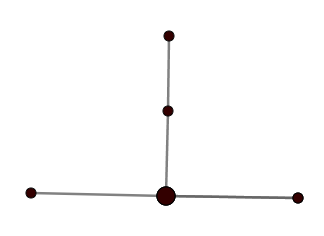
\includegraphics[width=0.35\linewidth]{image3.png}
\end{figure}
\textbf{Решение задачи.} Из предыдущего задани мы выяснили, что наша задача аппроксимируется разностной схемой с погрешностью $O(h+\tau^2)$ для самого уравнения и $O(\tau)$, $O(h)$ для начального и краевого условий соответственно. Нам необходимо за счет повышение порядка аппроксимации начального и краевого условий повысить порядок аппроксимации разностной схемы с $O(h+\tau)$ до $O(h^2+\tau^2)$. 

Для повышения порядка аппроксимации по времени, поднимем порядок аппроксимации второго начального условия, не расширяя шаблона, для этого будем искать новое разностное условие в следующем виде:
$$u_t(x,0)=\overline{u_1(x)},$$
Опеределим погрешность аппроксимации начального условия:
$$\nu(x,0)=u_t(x,0)-\overline{u_1(x)}=\frac{\partial u(x,0)}{\partial t}+\frac{\tau}{2}\frac{\partial^2 u(x,0)}{\partial t^2}+O(\tau^2)-\overline{u_1(x)}=u_1(x)+\frac{\tau}{2}\frac{\partial^2 u(x,0)}{\partial t^2}+O(\tau^2)-\overline{u_1(x)}.$$
Таким образом, в качестве $\overline{u_0(x)}$ можно взять, например,
$$\overline{u_1(x)}=u_1(x)+\frac{\tau}{2}\frac{\partial^2 u(x,0)}{\partial t^2}.$$
Для повышения порядка аппроксимации по $x$, поднимем порядок аппроксимации первого граничного условия, не расширяя шаблона, для этого будем искать новое разностное условие в следующем виде:
$$u_x(0,t)=\overline{\sigma_0}u(0,t)-\overline{\mu_0(t)}.$$
Определим погрешность аппроксимации:
$$\nu(0,t)=u_x(0,t)-\overline{\sigma_0}u(0,t)+\overline{\mu_0(t)}=\frac{\partial u(0,t)}{\partial x}+\frac{h}{2}\frac{\partial^2 u(0,t)}{\partial x^2}+O(h^2)-\overline{\sigma_0}u(0,t)+\overline{\mu_0(t)}=$$
$$=\sigma_0 u(0,t)-\mu_0(t)+\frac{h}{2}\frac{\partial^2 u(0,t)}{\partial x^2}+O(h^2)-\overline{\sigma_0}u(0,t)+\overline{\mu_0(t)}.$$
Таким образом, в качестве $\overline{\sigma_0}u(0,t)-\overline{\mu_0(t)}$ можно взять, например
$$\overline{\sigma_0}u(0,t)-\overline{\mu_0(t)}=\sigma_0 u(0,t)-\mu_0(t)+\frac{h}{2}\frac{\partial^2 u(0,t)}{\partial x^2}.$$
Выразим из уравнения исходной задачи 
$$\frac{\partial^2 u(0,t)}{\partial x^2}=\frac{\partial^2 u(0,t)}{\partial t^2}-q(x,0)u(x,0)-f(x,0)=\frac{\partial^2 u(0,t)}{\partial t^2}-q(x,0)u_0(x)-f(x,0)=-q(x,0)u_0(x)-f(x,0).$$
Тогда получим:
$$\overline{\sigma_0}u(0,t)-\overline{\mu_0(t)}=\sigma_0 u(0,t)-\mu_0(t)+\frac{h}{2}(\frac{\partial^2 u(0,t)}{\partial t^2}-q(x,0)u_0(x)-f(x,0)).$$
Таким образом, разностная схема второго порядка по $x$ и второго порядка по времени в индексной форме будет иметь вид:
$$\begin{cases}
    \frac{y_i^{j+2}-2y_i^{j+1}+y_{i}^j}{\tau^2}=\frac{y_{i+1}^j-2y_i^j+y_{i-1}^j}{h^2}+q(x_i,t_j)y_i^j+f(x_i,t_j),i=\overline{1,N-1},\\
    y_i^0=u_0(x_i),\\
    \frac{y_{i+1}^1-y_{i+1}^0}{h}=u_1(x)+\frac{y_i^{2}-2y_i^{1}+y_{i}^0}{2\tau},\\
    \frac{y_{1}^{j+1}-y_{0}^{j+1}}{h}=\sigma_0 y_0^{j}-\mu_0(t_j)+\frac{h}{2}(\frac{y_0^{j+2}-2y_0^{j+1}+y_{0}^j}{\tau^2}-q(x_i,0)u_0(x_i)-f(x_i,0)),\\
    y_{1}^{j+1}=\mu_1(t_j)
\end{cases}$$
\end{document}